\documentclass[12pt, a4paper]{article}

% --- Pakiety ---
\usepackage[utf8]{inputenc}
\usepackage[T1]{fontenc}
\usepackage[polish]{babel}
\usepackage{geometry}
\usepackage{amsmath}
\usepackage{amssymb}
\usepackage{graphicx}
\usepackage{booktabs}
\usepackage{siunitx}
\usepackage{caption}
\usepackage{subcaption}
\usepackage{float}
\usepackage{hyperref}
\usepackage{xcolor}
\usepackage{array}
\usepackage{multirow}
\usepackage{fancyhdr}

% --- Marginesy ---
\geometry{
    top=2.5cm,
    bottom=2.5cm,
    left=2.5cm,
    right=2.5cm
}

% --- Stopka ---
\pagestyle{fancy}
\fancyhf{}
\renewcommand{\headrulewidth}{0pt}
\renewcommand{\footrulewidth}{0.4pt}
\fancyfoot[R]{
\includegraphics[height=0.8cm]{lumon.pdf}}

% --- Konfiguracja siunitx ---
\sisetup{
    output-decimal-marker = {,},
    separate-uncertainty = true
}

% --- Dane raportu ---
\newcommand{\tytul}{Cechowanie termopary i termistora}
\newcommand{\codeword}{Adelaide}
\newcommand{\nrCwiczenia}{C1}
\newcommand{\autor}{Karol Peszek}
\newcommand{\nrGrupy}{B}
\newcommand{\dataWykonania}{11 marca 2026}

% --- Tytuł dokumentu ---
\title{
    \large I Pracownia Fizyczna \\[0.5em]
    \textbf{Ćwiczenie nr \nrCwiczenia} \\[0.3em]
    \LARGE \tytul\space''\codeword''
}
\author{
    \autor\\
     Grupa \nrGrupy}
\date{
    Data wykonania pomiarów: \dataWykonania\\
}

% =============================================
\begin{document}
% =============================================

\maketitle
\thispagestyle{empty}
\newpage

% -------------------------------------------
\section{Cel ćwiczenia}
% -------------------------------------------

Celem ćwiczenia jest zapoznanie się z mechanizmem działania termopary i
termistora, a następnie wyznaczenie eksperymentalne ich charakterystyk
temperaturowych. Po wyznaczeniu charakterystyk tych czujników celem ćwiczenia
będzie obliczenie szerokości pasma półprzewodniczego termistora.
% -------------------------------------------
\section{Wstęp teoretyczny}
% -------------------------------------------

\subsection{Zjawisko termoelektryczne}

Zjawisko termoelektryczne (efekt Seebecka) polega na powstawaniu siły
elektromotorycznej (SEM) w obwodzie złożonym z dwóch różnych przewodników lub
półprzewodników, których złącza (spoiny) znajdują się w różnych temperaturach.
Odkryte w 1821 roku przez Thomasa Johanna Seebecka, zjawisko to jest podstawą
działania \textbf{termopary}.

Gdy spoina gorąca (pomiarowa) znajduje się w temperaturze $T$, a spoina zimna
(referencyjna) w temperaturze $T_0$, w obwodzie pojawia się napięcie
termoelektryczne:
\begin{equation}
    U = \alpha (T_1 - T_2),
\end{equation}
gdzie $\alpha$ jest współczynnikiem Seebecka (termoelektrycznym) pary materiałów, wyrażonym w \si{m\volt\per\kelvin}.

W eksperymencie jeden z końców termopary umieszczony był w termosie z wodą i
lodem, zatem można przyjąć $T_2 = 0 \,^\circ\mathrm{C}$, a drugi w kąpieli
wodnej o zmiennej temperaturze $T_1$. Możemy zatem uprościć równanie do
postaci:
\begin{equation}
    U = \alpha T_1.
\end{equation}
\begin{equation}
    T_1 = \frac{U}{\alpha}.
    \label{thermocouple_linreg}
\end{equation}
Oznacza to, że napięcie termoelektryczne jest proporcjonalne do temperatury spoina gorącego, co pozwala na wyznaczenie charakterystyki termopary poprzez pomiar napięcia przy różnych temperaturach.

\subsection{Termistor}

\textbf{Termistor} jest elementem półprzewodnikowym, którego rezystancja silnie zależy od temperatury. W odróżnieniu od metali, w których rezystancja rośnie wraz z temperaturą, termistory NTC (\textit{Negative Temperature Coefficient}) wykazują jej gwałtowny spadek.

Zachowanie termistora NTC opisuje \textbf{równanie Steinhart-Harta}, jednak w
praktyce laboratoryjnej stosuje się prostszą zależność wynikającą z modelu
pasmowego półprzewodnika. Przewodnictwo elektryczne półprzewodnika zależy
eksponencjalnie od temperatury przez czynnik Boltzmanna:
\begin{equation}
    R(T) = R_0 \exp\!\left(\frac{W}{2k_B T}\right),
    \label{eq:termistor}
\end{equation}
gdzie $R_0$ jest stałą materiałową, $W$ — szerokością przerwy energetycznej (pasma wzbronionego) półprzewodnika, $k_B = \SI{8.617e-5}{\electronvolt\per\kelvin}$ — stałą Boltzmanna, a $T$ — temperaturą bezwzględną.

Linearyzując równanie~\eqref{eq:termistor} przez zlogarytmowanie obu stron,
otrzymuje się:
\begin{equation}
    \ln R = \ln R_0 + \frac{W}{2k_B} \cdot \frac{1}{T}.
    \label{eq:termistor_lin}
\end{equation}
Po elementarnych przekształceniach:
\begin{equation}
    \frac{1}{T} = \frac{2k_B}{W} \ln R - \frac{2k_B}{W} \ln R_0
\end{equation}
% -------------------------------------------
\section{Opis układu pomiarowego}
% -------------------------------------------

\begin{figure}[H]
    \centering
    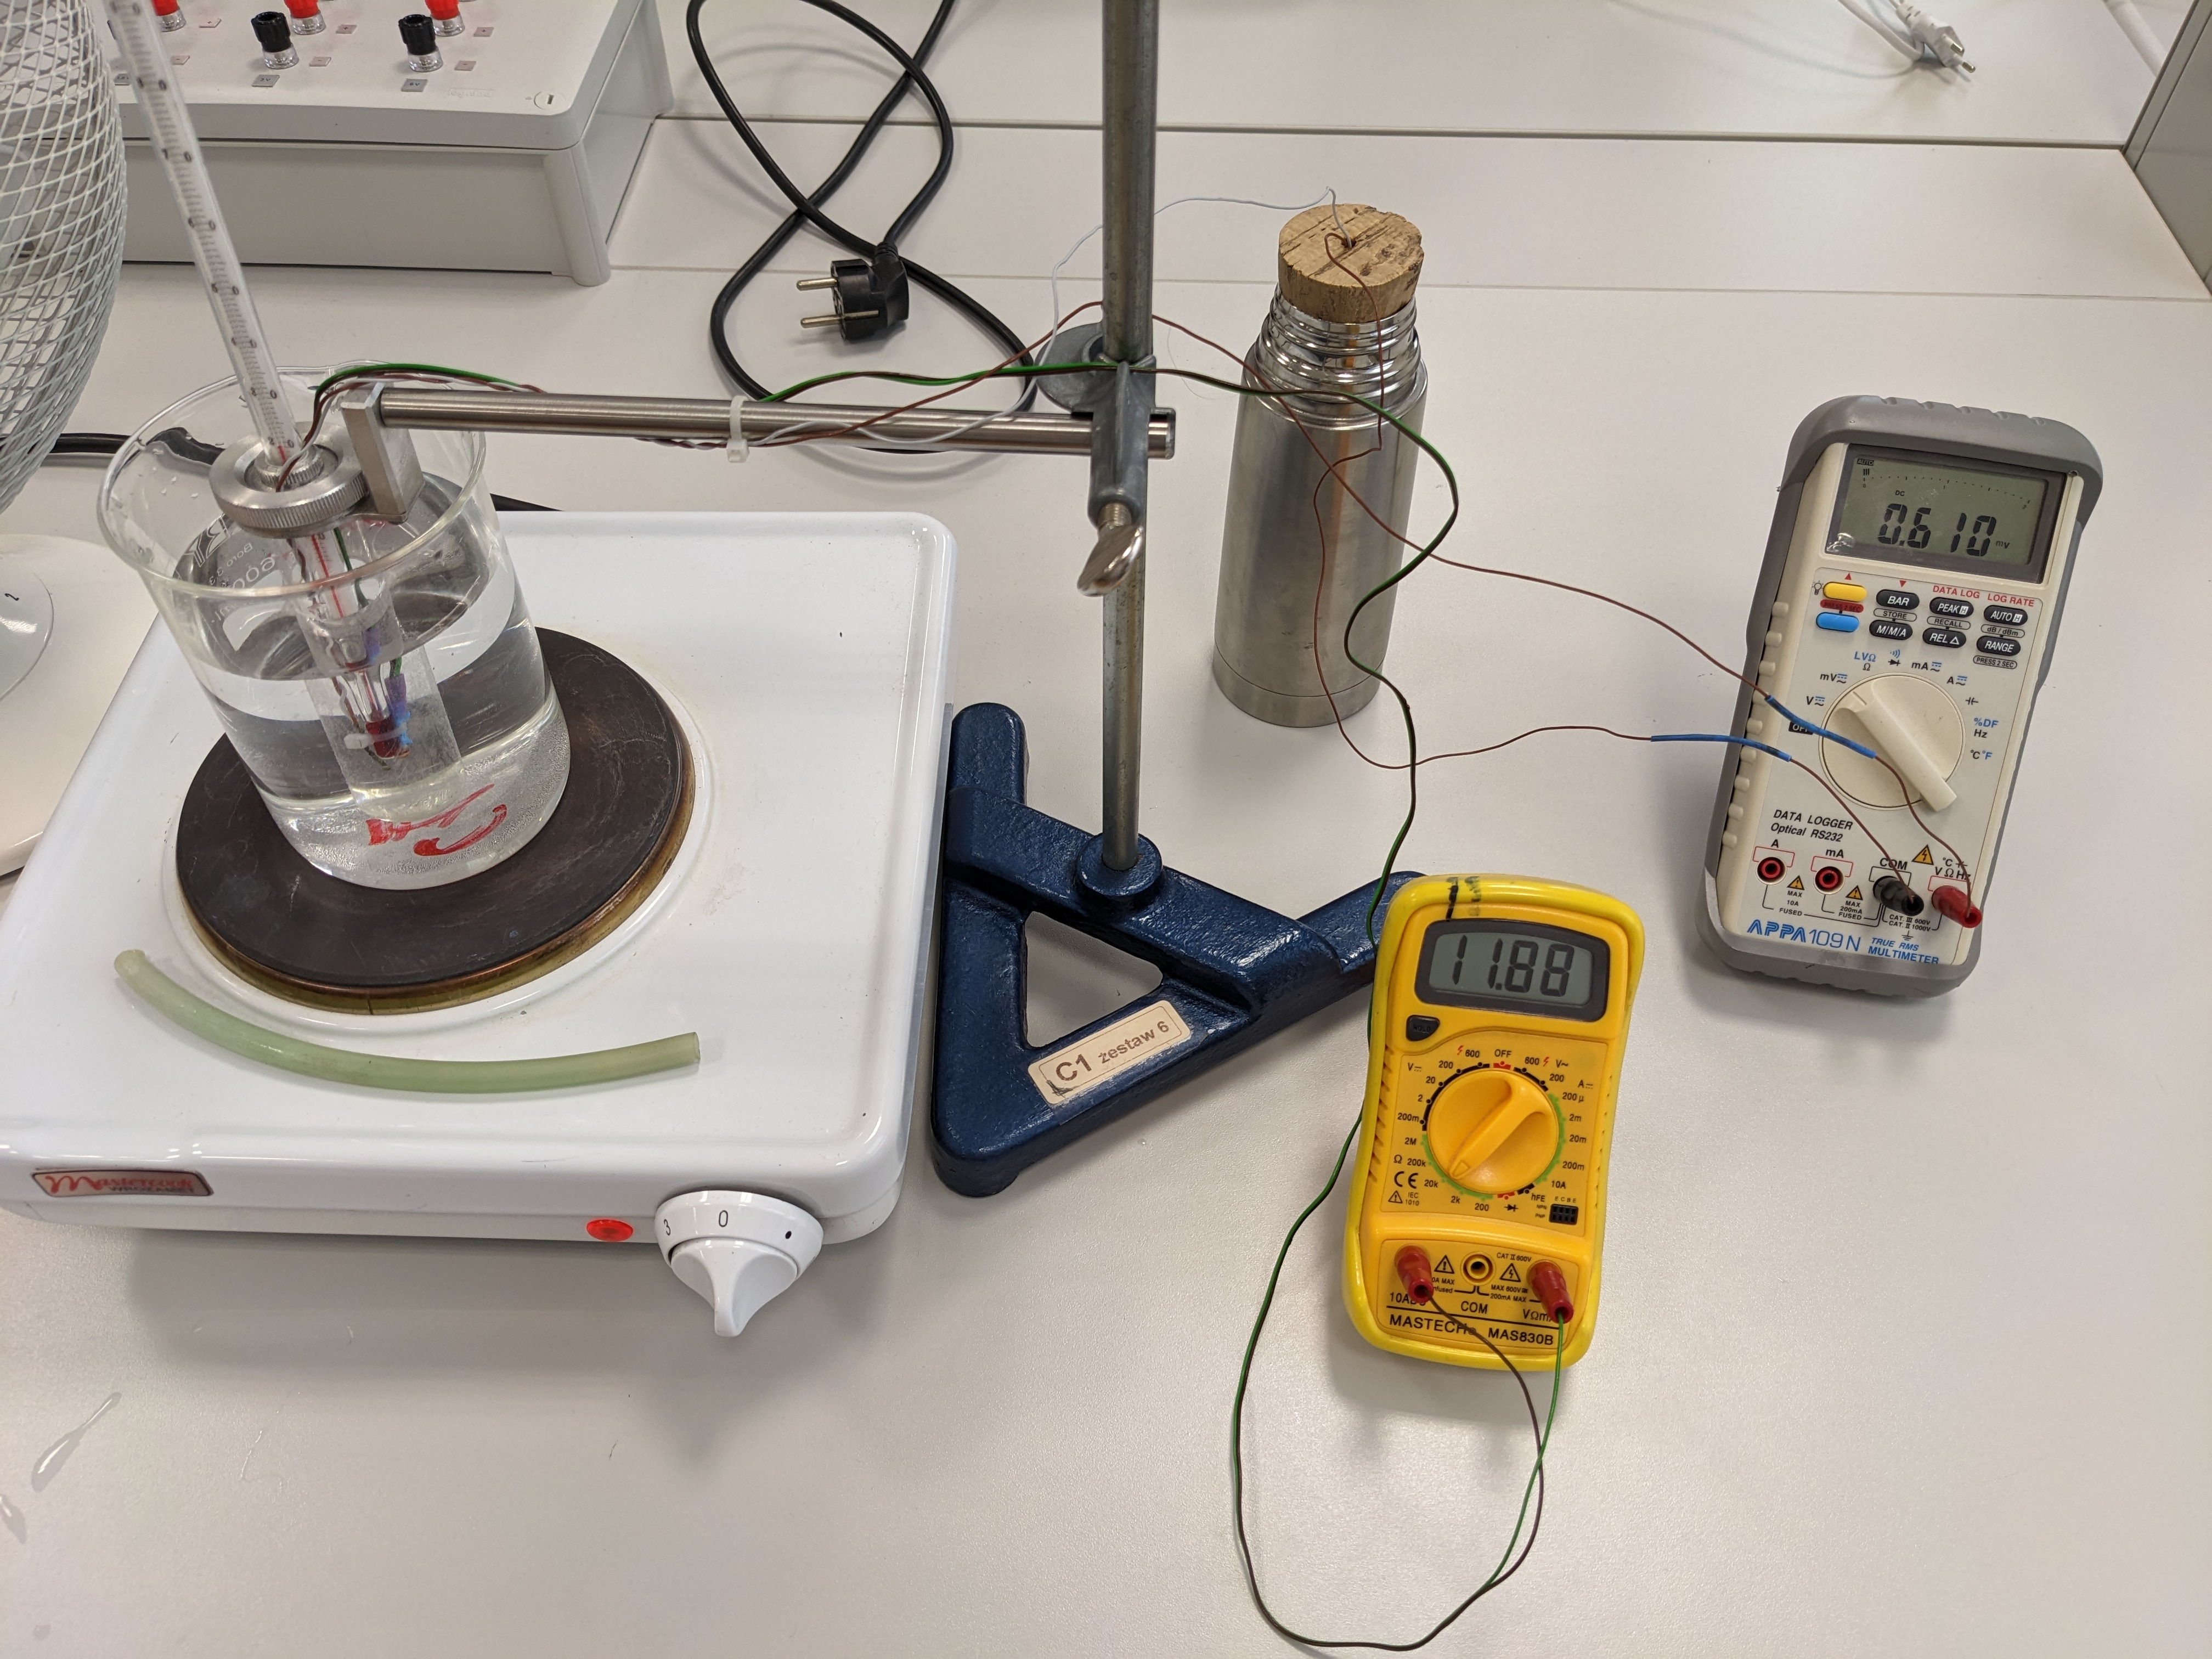
\includegraphics[width=1\textwidth]{schema.jpg}
    \caption{Schemat układu pomiarowego.}\label{fig:schemat}
\end{figure}
s
\subsection{Przyrządy użyte do przeprowadzenia eksperymentu}
\begin{itemize}
    \item miliwoltomierz APPA 109N (dokładność: \SI{\pm0.06}{\percent})
    \item omomierz Mastech MAS830B (dokładność: \SI{\pm0.08}{\percent})
    \item kuchenka z regulacją temperatury
    \item zlewka z wodą
    \item termos z wodą i lodem oraz korkiem izolacyjnym
    \item stojak z uchwytem do termopary i termistora
    \item gumowy wężyk do mieszania wody
    \item termometr rtęciowy (dokładność: \SI{\pm0.5}{\degreeCelsius})
    \item termopara
    \item termistor typu NTC
\end{itemize}

\subsection{Opis układu}
Na stojaku zamocowany jest uchwyt trzymający fiolkę wypełnioną olejem
nieprzewodzącym prądu, w której umieszczone są końcówki termopary i termistora.
Fiolka jest zanurzona w zlewce z wodą, której temperaturę można regulować za
pomocą kuchenki. Termos z wodą i lodem służy do utrzymania stałej temperatury
odniesienia dla termopary. Miliwoltomierz służy do pomiaru napięcia
termoelektrycznego generowanego przez termoparę, natomiast omomierz do pomiaru
rezystancji termistora. Termometr rtęciowy jest używany do kontrolowania
temperatury w zlewce, a gumowy wężyk do mieszania wody, zapewniając równomierną
temperaturę w całej objętości.
% -------------------------------------------
\section{Procedura pomiarowa}
Pomiary przeprowadzono w dniu 11.03.2026 roku. Procedura pomiarowa była
następująca:
\begin{enumerate}
    \item Przygotowanie układu pomiarowego zgodnie ze schematem na
          zdjęciu~\ref{fig:schemat}.
    \item Ustawienie termopary i termistora w fiolce z olejem, a następnie zanurzenie
          fiolki w zlewce z wodą.
    \item Rozpoczęcie podgrzewania wody w zlewce za pomocą kuchenki, jednocześnie
          mieszając wodę wężem, aby zapewnić równomierną temperaturę.
    \item W trakcie podgrzewania, notowanie co $2 \,^\circ\mathrm{C}$ naprzemiennie
          odczytów z termometru rtęciowego, napięcia z termopary oraz rezystancji
          termistora.
    \item Kontynuowanie pomiarów aż do osiągnięcia temperatury $93 \,^\circ\mathrm{C}$.
          Dalsze podgrzewanie nie było możliwe ze względu na ograniczenia sprzętowe.
    \item Po zakończeniu pomiarów, wyłączenie kuchenki i wyjęcie fiolki z gorącej wody.
    \item Notowanie odczytów również co $2 \,^\circ\mathrm{C}$ podczas schładzania wody,
          aż do osiągnięcia temperatury około $20 \,^\circ\mathrm{C}$.
\end{enumerate}
% -------------------------------------------
\section{Wyniki pomiarów}
% -------------------------------------------
Szczegółowe wyniki pomiarów znajdują się w zeszycie pomiarowym oraz w
dostarczonych plikach csv.

\subsection{Surowe wyniki pomiarów}
Wyniki podzielono na 4 części odpowiadające odpowiednio ogrzewaniu i chłodzeniu
termopary i termistora. Wyniki można zobaczyć na wykresie poniżej.

\begin{figure}[H]
    \centering
    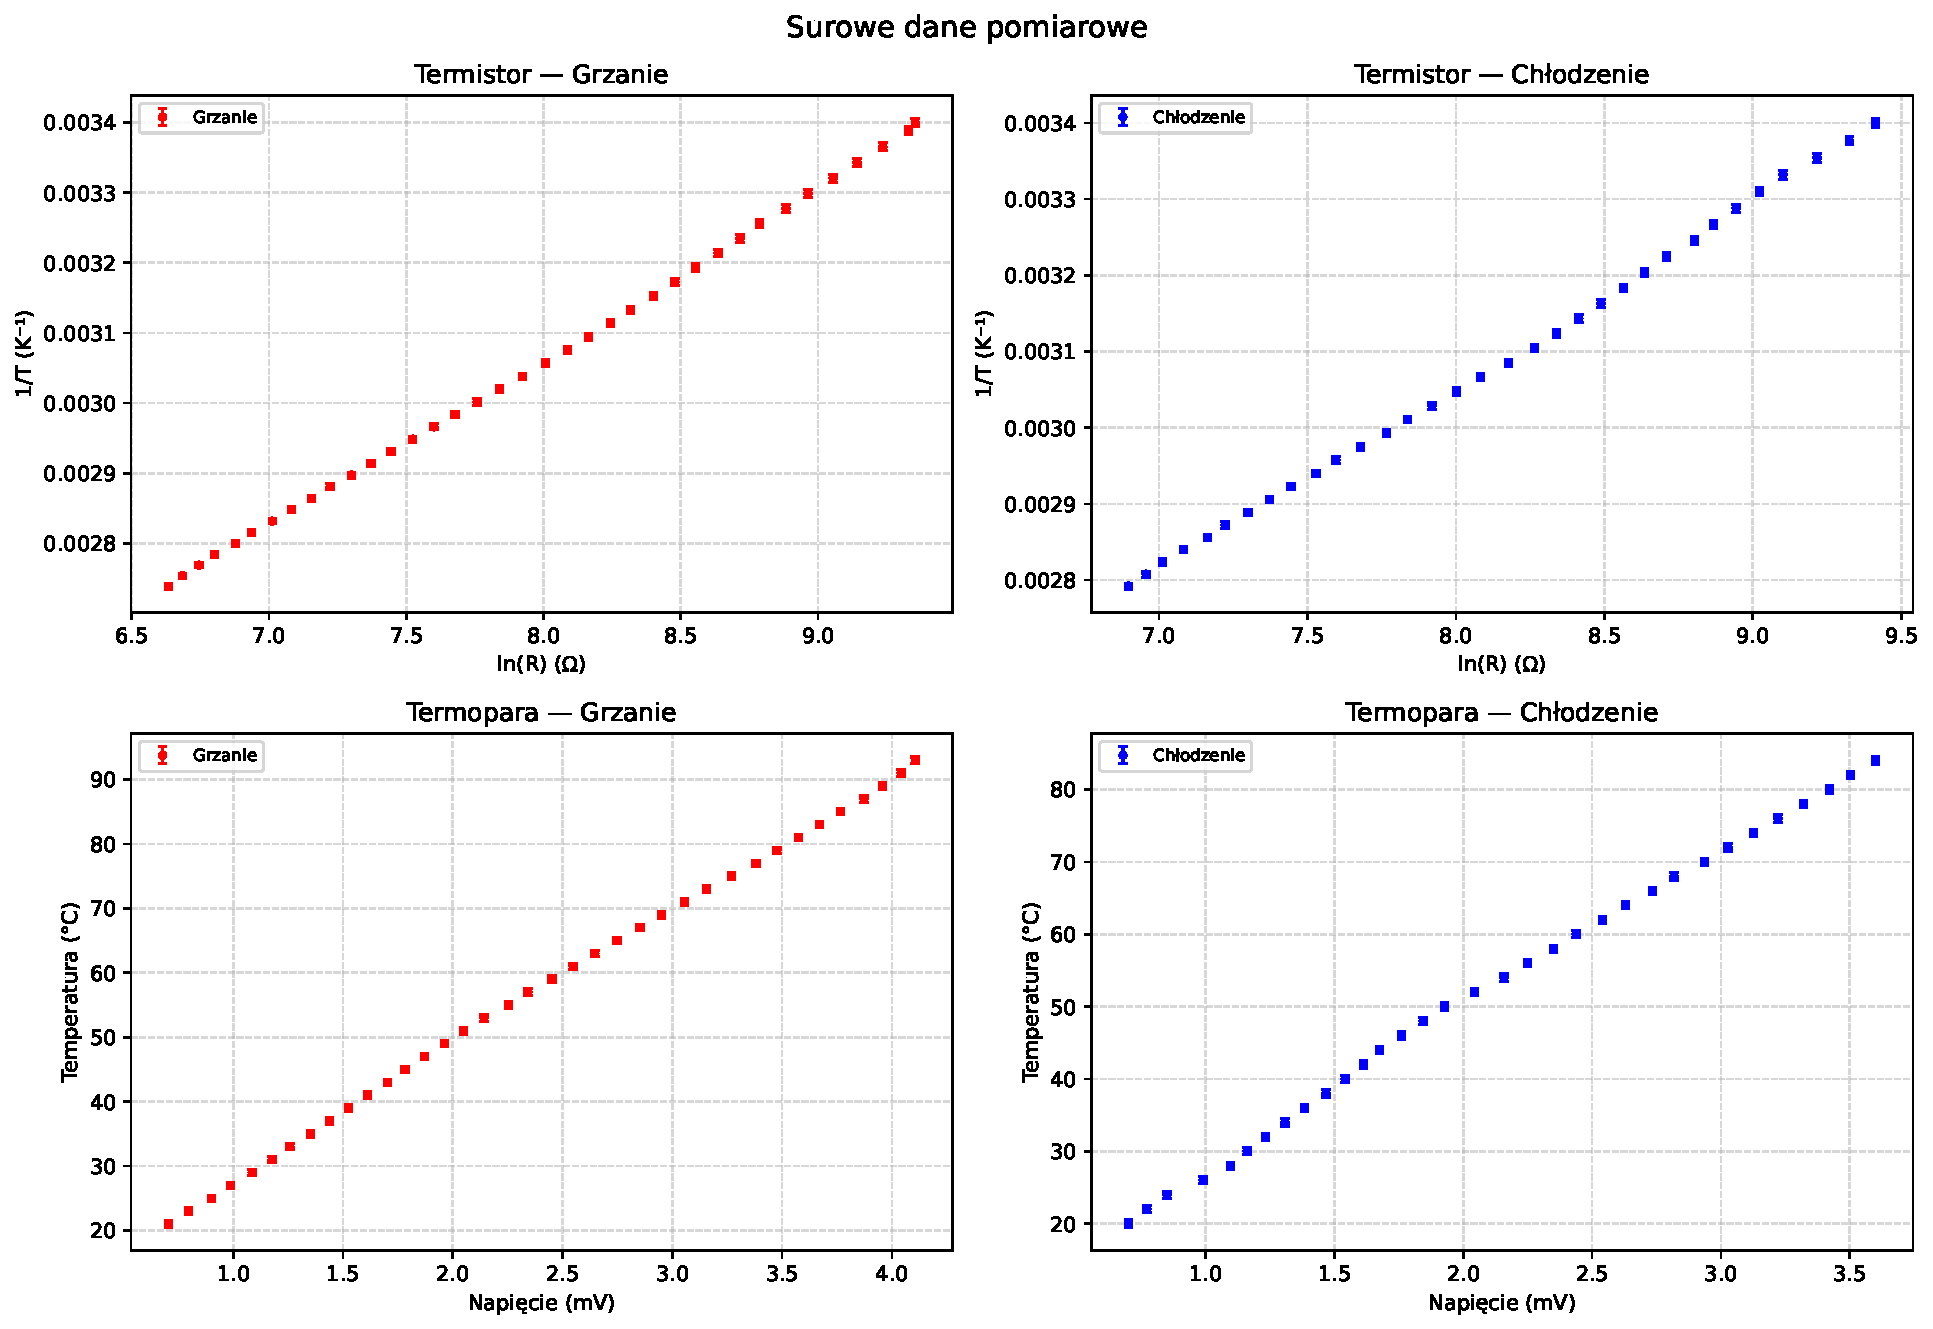
\includegraphics[width=0.9\textwidth]{wykres0_surowe_dane.pdf}
    \caption{Surowe wyniki pomiarów: temperatura wewnątrz fiolki z olejem w funkcji napięcia termopary i rezystancji termistora. Ogrzewanie i chłodzenie przedstawione są oddzielnie.}\label{fig:surowe_dane}
\end{figure}

\subsection{Użyte modele regresji}
Jak widać z wykresów dane nie układają się idealnie na prostej. Przeprowadzono
zatem różne rodzaje regresji liniowej, w tym:
\begin{enumerate}
    \item Dla termopary --- model liniowy $T = aU + b$:
          \begin{itemize}
              \item Regresja \textbf{zakotwiczona} w $T_0 = 0\,^\circ\mathrm{C}$ (spoina zimna w
                    termosie z lodem): model $T = aU + T_0$, gdzie wyraz wolny jest ustalony.
                    Przeprowadzona osobno dla pierwszej i drugiej połowy grzania oraz chłodzenia, a
                    także dla danych łączonych.
              \item Regresja \textbf{swobodna} (bez kotwiczenia): model $T = aU + b$, gdzie oba
                    współczynniki są dopasowywane. Przeprowadzona osobno dla pierwszej i drugiej
                    połowy grzania oraz chłodzenia, a także dla danych łączonych.
          \end{itemize}
    \item Dla termistora --- linearyzacja modelu wykładniczego\eqref{eq:termistor} przez
          podstawienie $x = \ln R$, $y = 1/T$:
          \begin{itemize}
              \item Regresja \textbf{swobodna}: model $\frac{1}{T} = a \ln R + b$. Przeprowadzona
                    dla wszystkich danych z grzania, wszystkich danych z chłodzenia, danych
                    łączonych, a także osobno dla pierwszej i drugiej połowy każdego zestawu.
          \end{itemize}
\end{enumerate}

\subsection{Wyniki regresji}
Wyniki regresji przedstawiono w tabeli~\ref{tab:regresja}.

\begin{table}[H]
    \centering
    \footnotesize
    \setlength{\tabcolsep}{4pt}
    \caption{Wyniki regresji liniowej dla termopary i termistora.}\label{tab:regresja}
    \resizebox{\textwidth}{!}{%
        \begin{tabular}{llllllll}
            \toprule
            Czujnik & Zestaw     & Połowa    & Model                      & Zakotwiczony                      & $a \pm u(a)$                    & $b \pm u(b)$                    \\
            \midrule
            \multirow{7}{*}{Termistor}
                    & Grzanie    & wszystkie & $\frac{1}{T} = a\ln R + b$ & Nie                               & $\num{2.4e-4} \pm \num{1.1e-6}$ & $\num{1.2e-3} \pm \num{8.6e-6}$ \\
                    & Chłodzenie & wszystkie & $\frac{1}{T} = a\ln R + b$ & Nie                               & $\num{2.4e-4} \pm \num{1.6e-6}$ & $\num{1.1e-3} \pm \num{1.3e-5}$ \\
                    & Łączone    & ---       & $\frac{1}{T} = a\ln R + b$ & Nie                               & $\num{2.4e-4} \pm \num{1.2e-6}$ & $\num{1.1e-3} \pm \num{9.7e-6}$ \\
                    & Grzanie    & 1.\ poł.  & $\frac{1}{T} = a\ln R + b$ & Nie                               & $\num{2.3e-4} \pm \num{1.1e-6}$ & $\num{1.2e-3} \pm \num{7.6e-6}$ \\
                    & Grzanie    & 2.\ poł.  & $\frac{1}{T} = a\ln R + b$ & Nie                               & $\num{2.5e-4} \pm \num{9.1e-7}$ & $\num{1.0e-3} \pm \num{7.9e-6}$ \\
                    & Chłodzenie & 1.\ poł.  & $\frac{1}{T} = a\ln R + b$ & Nie                               & $\num{2.3e-4} \pm \num{1.3e-6}$ & $\num{1.2e-3} \pm \num{9.4e-6}$ \\
                    & Chłodzenie & 2.\ poł.  & $\frac{1}{T} = a\ln R + b$ & Nie                               & $\num{2.6e-4} \pm \num{2.5e-6}$ & $\num{9.7e-4} \pm \num{2.2e-5}$ \\
            \midrule
            \multirow{12}{*}{Termopara}
                    & Grzanie    & 1.\ poł.  & $T = aU + T_0$             & Tak ($T_0 = 0\,^\circ\mathrm{C}$) & $\num{25}   \pm \num{0.23}$     & ---                             \\
                    & Grzanie    & 1.\ poł.  & $T = aU + b$               & Nie                               & $\num{22}   \pm \num{0.11}$     & $\num{4.9} \pm \num{0.16}$      \\
                    & Grzanie    & 2.\ poł.  & $T = aU + T_0$             & Tak ($T_0 = 0\,^\circ\mathrm{C}$) & $\num{23}   \pm \num{0.12}$     & ---                             \\
                    & Grzanie    & 2.\ poł.  & $T = aU + b$               & Nie                               & $\num{20}   \pm \num{0.15}$     & $\num{10}  \pm \num{0.49}$      \\
                    & Chłodzenie & 1.\ poł.  & $T = aU + T_0$             & Tak ($T_0 = 0\,^\circ\mathrm{C}$) & $\num{26}   \pm \num{0.15}$     & ---                             \\
                    & Chłodzenie & 1.\ poł.  & $T = aU + b$               & Nie                               & $\num{25}   \pm \num{0.42}$     & $\num{2}   \pm \num{0.59}$      \\
                    & Chłodzenie & 2.\ poł.  & $T = aU + T_0$             & Tak ($T_0 = 0\,^\circ\mathrm{C}$) & $\num{24}   \pm \num{0.14}$     & ---                             \\
                    & Chłodzenie & 2.\ poł.  & $T = aU + b$               & Nie                               & $\num{21}   \pm \num{0.069}$    & $\num{9.7} \pm \num{0.2}$       \\
                    & Łączone    & 1.\ poł.  & $T = aU + T_0$             & Tak ($T_0 = 0\,^\circ\mathrm{C}$) & $\num{26}   \pm \num{0.16}$     & ---                             \\
                    & Łączone    & 1.\ poł.  & $T = aU + b$               & Nie                               & $\num{23}   \pm \num{0.27}$     & $\num{3.9} \pm \num{0.4}$       \\
                    & Łączone    & 2.\ poł.  & $T = aU + T_0$             & Tak ($T_0 = 0\,^\circ\mathrm{C}$) & $\num{23}   \pm \num{0.12}$     & ---                             \\
                    & Łączone    & 2.\ poł.  & $T = aU + b$               & Nie                               & $\num{20}   \pm \num{0.25}$     & $\num{12}  \pm \num{0.76}$      \\
            \bottomrule
        \end{tabular}%
    }
\end{table}

Na wykresach~\ref{fig:termistor_pelne}--\ref{fig:termopara_laczone}
przedstawiono graficznie wszystkie przeprowadzone regresje. Każdy punkt danych
zaznaczono czarnym kółkiem z słupkami błędów. Dla termistora słupki pionowe
odpowiadają niepewności $u(1/T) = u(T)/T^2$, gdzie $u(T) = \SI{0.5}{\kelvin}$
pochodzi od dokładności termometru rtęciowego. Dla termopary słupki pionowe
odpowiadają bezpośredniej niepewności odczytu temperatury $u(T) =
    \SI{0.5}{\degreeCelsius}$. Zacieniowany obszar wokół każdej prostej jest
przedziałem niepewności wartości dopasowanej $u(\hat{y}) = \sqrt{{\bigl(x\cdot
            u(a)\bigr)}^2 + {u(b)}^2}$, wyznaczonym przez propagację niepewności
współczynników regresji; dla modelu zakotwiczonego (termopara, linia
przerywana) wyraz wolny jest stały, więc $u(\hat{T}) = |U|\cdot u(a)$.

% Termistor: pełne zestawy danych (grzanie, chłodzenie, łączone)
\begin{figure}[H]
    \centering
    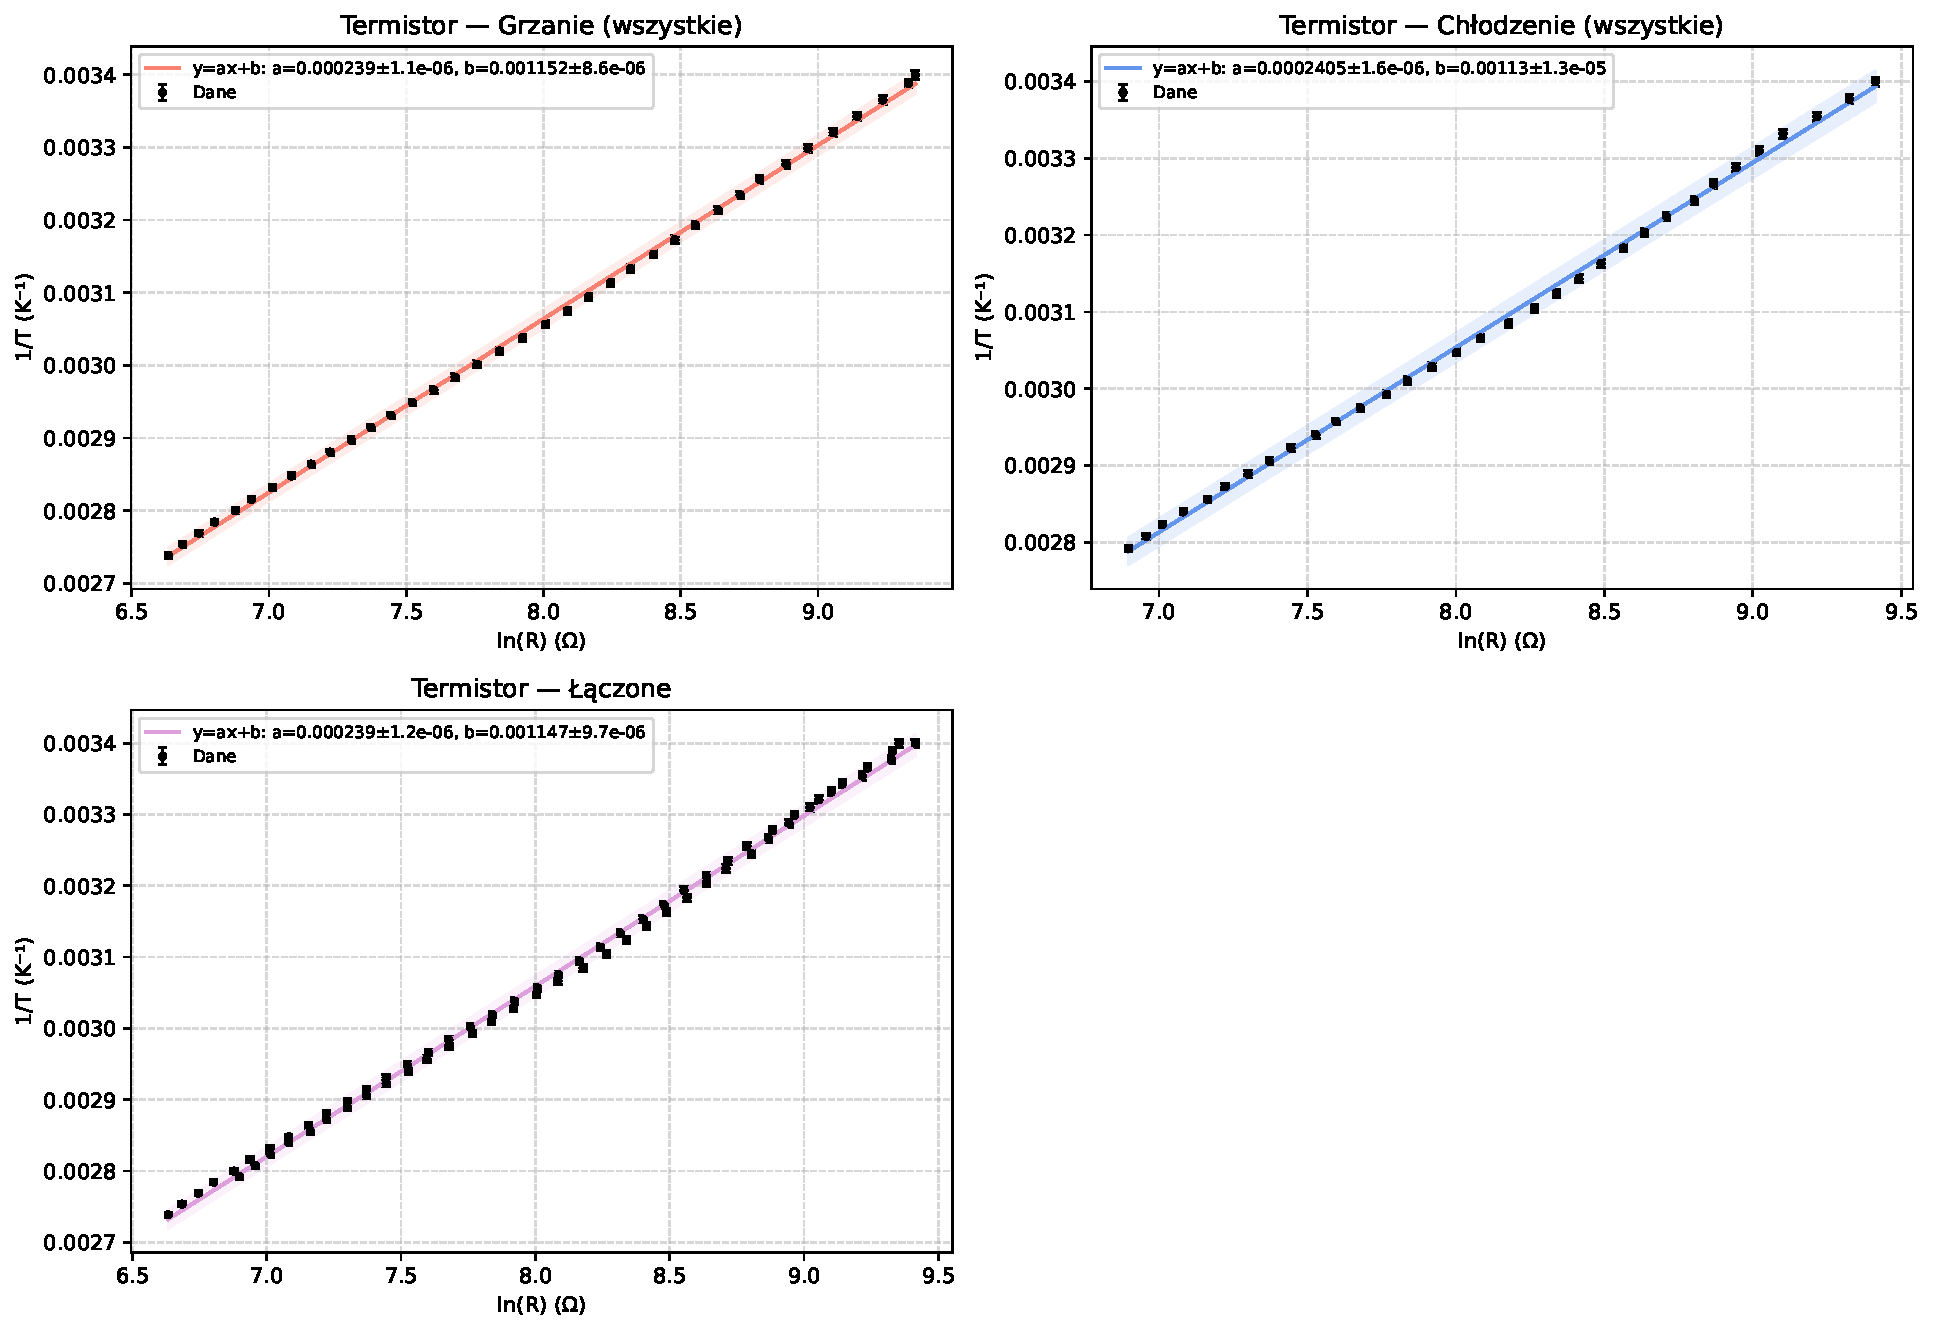
\includegraphics[width=0.95\textwidth]{wykres1_termistor_pelne.pdf}
    \caption{Regresja liniowa termistora --- model $1/T = a\ln R + b$ --- dla trzech pełnych zestawów
        danych: grzania (czerwony), chłodzenia (niebieski) i danych łączonych (fioletowy).
        Oś~$x$: $\ln R$ (rezystancja $R$ w $\Omega$); oś~$y$: $1/T$ (temperatura $T$ w~K).
        Linia ciągła --- dopasowana prosta MNK;\@ zacieniowany obszar --- niepewność wartości
        dopasowanej wynikająca z niepewności współczynników $u(a)$ i $u(b)$.
        Nachylenie $a = W/(2k_B)$ pozwala wyznaczyć szerokość przerwy energetycznej
        półprzewodnika $W = 2k_B/a$.}\label{fig:termistor_pelne}
\end{figure}

% Termistor: dane podzielone na pierwszą i drugą połowę każdego zestawu
\begin{figure}[H]
    \centering
    
\includegraphics[width=0.95\textwidth]{wykres2_termistor_polowy.pdf}
    \caption{Regresja liniowa termistora dla pierwszej i drugiej połowy zestawów grzania
        (czerwony) oraz chłodzenia (niebieski).
        Podział przeprowadzono przez posortowanie danych względem $\ln R$
        i podzielenie na dwie równoliczne grupy, co odpowiada rozdzieleniu zakresu niskich
        i wysokich temperatur.
        Osie, linia i zacieniowany obszar jak na rys.~\ref{fig:termistor_pelne}.
        Różnice nachyleń między połówkami wskazują na ewentualną nieliniowość
        lub ewentualne błędy/ograniczenia pomiarowe.}\label{fig:termistor_polowy}
\end{figure}

% Termopara: połowy zestawów grzania i chłodzenia
\begin{figure}[H]
    \centering
    
\includegraphics[width=0.95\textwidth]{wykres3_termopara_polowy.pdf}
    \caption{Regresja liniowa termopary dla pierwszej i drugiej połowy zestawów grzania
    (czerwony) oraz chłodzenia (niebieski).
    Oś~$x$: napięcie termoelektryczne $U$ (mV); oś~$y$: temperatura $T$ (\si{\degreeCelsius}).
    Linia przerywana --- model zakotwiczony $T = aU + T_0$ z ustalonym wyrazem wolnym
    $T_0 = 0\,^\circ\mathrm{C}$ (spoina zimna w termosie z lodem);
    zacieniowany obszar wokół linii przerywanej --- $u(\hat{T}) = |U|\cdot u(a)$
    (niepewność pochodzi wyłącznie od $u(a)$, bo $T_0$ jest stałe).
    Linia ciągła --- model swobodny $T = aU + b$;
    zacieniowany obszar wokół linii ciągłej --- $u(\hat{T}) = \sqrt{{(U\cdot u(a))}^2 + {(u(b))}^2}$.
    Niezerowy wyraz wolny $b$ w modelu swobodnym sygnalizuje
    odchylenie od idealnego zachowania lub błąd systematyczny układu.}\label{fig:termopara_polowy}
\end{figure}

% Termopara: dane łączone (grzanie + chłodzenie)
\begin{figure}[H]
    \centering
    
\includegraphics[width=0.95\textwidth]{wykres4_termopara_laczone.pdf}
    \caption{Regresja liniowa termopary dla danych łączonych (grzanie i chłodzenie razem),
        osobno dla pierwszej i drugiej połowy zakresu temperatur.
        Osie, linia przerywana (model zakotwiczony) i linia ciągła (model swobodny)
        oraz zacieniowane obszary jak na rys.~\ref{fig:termopara_polowy}.
        Połączenie obu serii zwiększa liczbę punktów, co zmniejsza niepewności
        współczynników regresji. Porównanie wyników z rys.~\ref{fig:termopara_polowy}
        pozwala ocenić powtarzalność i symetrię charakterystyki termopary
        podczas grzania i chłodzenia.}\label{fig:termopara_laczone}
\end{figure}

\section{Opracowanie wyników}
\subsection{Obliczenia szerokości pasma półprzewodniczego termistora}
Celem zadania było nie tylko wyznaczenie charakterystyk termopary i termistora,
ale także obliczenie szerokości pasma półprzewodniczego $W$ termistora. Zrobimy
to w oparciu o różne modele regresji. Następnie wyliczymy ostateczne wyniki
jako średnie ważone, gdzie wagami będą odwrotności niepewności $u(a)$, a także
ocenimy niepewność ostatecznego wyniku $W$ poprzez propagację niepewności z
$a$.

Mając wyznaczone wartości współczynnika $a$ z różnych modeli regresji, możemy
obliczyć szerokość pasma półprzewodniczego $W$ dla każdego modelu:
\begin{equation}
    W = \frac{2k_B}{a}.
\end{equation}

Niepewność $u(W)$ dla każdego modelu można obliczyć przez propagację
niepewności z $a$:
\begin{equation}
    u(W) = \left| \frac{\partial W}{\partial a} \right| u(a) = \frac{2k_B}{a^2} u(a).
\end{equation}

Szerokość pasma półprzewodniczego $W$ dla każdego modelu wraz z niepewnością
$u(W)$ znajduje się w tabeli~\ref{tab:W}.

\begin{table}[H]
    \centering
    \caption{Przerwa energetyczna $W$ termistora wyznaczona z modelu $1/T = a\ln R + b$, wzór $W = 2k_B/a$.}\label{tab:W}
    \sisetup{separate-uncertainty=false}
    \begin{tabular}{l
            S[table-format=1.4e-1] @{${}\pm{}$} S[table-format=1.1e-1]
            S[table-format=1.4]    @{${}\pm{}$} S[table-format=1.4]}
        \toprule
        Zestaw
                               & \multicolumn{2}{c}{$a$ (\si{\per\kelvin})}
                               & \multicolumn{2}{c}{$W$ (\si{\electronvolt})}                            \\
        \midrule
        Grzanie (wszystkie)    & 2.390e-4                                     & 1.1e-6 & 0.7210 & 0.0033 \\
        Chłodzenie (wszystkie) & 2.405e-4                                     & 1.6e-6 & 0.7166 & 0.0048 \\
        Łączone                & 2.390e-4                                     & 1.2e-6 & 0.7210 & 0.0036 \\
        Grzanie 1.\ połowa     & 2.306e-4                                     & 1.1e-6 & 0.7474 & 0.0034 \\
        Grzanie 2.\ połowa     & 2.528e-4                                     & 9.1e-7 & 0.6816 & 0.0024 \\
        Chłodzenie 1.\ połowa  & 2.286e-4                                     & 1.3e-6 & 0.7540 & 0.0042 \\
        Chłodzenie 2.\ połowa  & 2.589e-4                                     & 2.5e-6 & 0.6657 & 0.0065 \\
        \bottomrule
    \end{tabular}
\end{table}

Biorąc pod uwagę wszystkie modele, możemy obliczyć średnią ważoną szerokości
pasma półprzewodniczego $W$:
\begin{equation}
    \bar{W} = \frac{\sum_i W_i / u^2(W_i)}{\sum_i 1 / u^2(W_i)}.
\end{equation}
Niepewność średniej ważonej $u(\bar{W})$ można obliczyć jako:
\begin{equation}
    u(\bar{W}) = \sqrt{\frac{1}{\sum_i 1 / u^2(W_i)}}.
\end{equation}

Podstawiając uzyskane wyniki do powyższych równań otrzymano następujące wyniki
dla szerokości pasma półprzewodniczego termistora:
\begin{equation}
    \bar{W} = \SI{0.7138}{\electronvolt} \pm \SI{0.0014}{\electronvolt}.
\end{equation}

\subsection{Obliczanie współczynnika Seebecka termopary}
Współczynnik Seebecka $\alpha$ dla termopary można obliczyć na podstawie
nachylenia $a$ z modelu zakotwiczonego $T = aU + T_0$, gdzie $T_0 =
    0\,^\circ\mathrm{C}$:
\begin{equation}
    \alpha = \frac{1}{a}.
\end{equation}
Niepewność $u(\alpha)$ można obliczyć przez propagację niepewności z $a$:
\begin{equation}
    u(\alpha) = \left| \frac{\partial \alpha}{\partial a} \right| u(a) = \frac{1}{a^2} u(a).
\end{equation}

Wyniki obliczone dla poszczególnych modeli zakotwiczonych termopary
przedstawiono w tabeli~\ref{tab:alpha}.

\begin{table}[H]
    \centering
    \footnotesize
    \sisetup{separate-uncertainty=false}
    \caption{Współczynnik Seebecka $\alpha$ termopary wyznaczony z modelu zakotwiczonego $T = aU + T_0$, wzór $\alpha = 1/a$.}\label{tab:alpha}
    \begin{tabular}{l
            S[table-format=2.2] @{${}\pm{}$} S[table-format=1.2]
            S[table-format=1.5] @{${}\pm{}$} S[table-format=1.5]
            S[table-format=2.2] @{${}\pm{}$} S[table-format=1.2]}
        \toprule
        Zestaw
                                  & \multicolumn{2}{c}{$a$ (\si{\degreeCelsius\per\milli\volt})}
                                  & \multicolumn{2}{c}{$\alpha$ (\si{\milli\volt\per\degreeCelsius})}
                                  & \multicolumn{2}{c}{$\alpha$ (\si{\micro\volt\per\degreeCelsius})}                                           \\
        \midrule
        Grzanie --- 1.\ połowa    & 25.42                                                             & 0.23 & 0.03934 & 0.00036 & 39.34 & 0.36 \\
        Grzanie --- 2.\ połowa    & 22.95                                                             & 0.12 & 0.04358 & 0.00023 & 43.58 & 0.23 \\
        Chłodzenie --- 1.\ połowa & 26.16                                                             & 0.15 & 0.03823 & 0.00022 & 38.23 & 0.22 \\
        Chłodzenie --- 2.\ połowa & 23.93                                                             & 0.14 & 0.04179 & 0.00025 & 41.79 & 0.25 \\
        Łączone --- 1.\ połowa    & 25.73                                                             & 0.16 & 0.03887 & 0.00024 & 38.87 & 0.24 \\
        Łączone --- 2.\ połowa    & 23.34                                                             & 0.12 & 0.04284 & 0.00022 & 42.84 & 0.22 \\
        \bottomrule
    \end{tabular}
\end{table}

Analogicznie, współczynnik Seebecka można wyznaczyć z modelu swobodnego
(niezakotwiczonego) $T = aU + b$, korzystając z tego samego wzoru $\alpha =
    1/a$. Wyniki przedstawiono w tabeli~\ref{tab:alpha_niezak}.

\begin{table}[H]
    \centering
    \footnotesize
    \sisetup{separate-uncertainty=false}
    \caption{Współczynnik Seebecka $\alpha$ termopary wyznaczony z modelu niezakotwiczonego $T = aU + b$, wzór $\alpha = 1/a$.}\label{tab:alpha_niezak}
    \begin{tabular}{l
            S[table-format=2.2] @{${}\pm{}$} S[table-format=1.3]
            S[table-format=1.5] @{${}\pm{}$} S[table-format=1.5]
            S[table-format=2.2] @{${}\pm{}$} S[table-format=1.2]}
        \toprule
        Zestaw
                                  & \multicolumn{2}{c}{$a$ (\si{\degreeCelsius\per\milli\volt})}
                                  & \multicolumn{2}{c}{$\alpha$ (\si{\milli\volt\per\degreeCelsius})}
                                  & \multicolumn{2}{c}{$\alpha$ (\si{\micro\volt\per\degreeCelsius})}                                            \\
        \midrule
        Grzanie --- 1.\ połowa    & 22.39                                                             & 0.11  & 0.04467 & 0.00021 & 44.67 & 0.21 \\
        Grzanie --- 2.\ połowa    & 19.94                                                             & 0.15  & 0.05015 & 0.00037 & 50.15 & 0.37 \\
        Chłodzenie --- 1.\ połowa & 24.73                                                             & 0.42  & 0.04044 & 0.00069 & 40.44 & 0.69 \\
        Chłodzenie --- 2.\ połowa & 20.59                                                             & 0.069 & 0.04857 & 0.00016 & 48.57 & 0.16 \\
        Łączone --- 1.\ połowa    & 23.17                                                             & 0.27  & 0.04316 & 0.00051 & 43.16 & 0.51 \\
        Łączone --- 2.\ połowa    & 19.65                                                             & 0.25  & 0.05088 & 0.00064 & 50.88 & 0.64 \\
        \bottomrule
    \end{tabular}
\end{table}

Biorąc pod uwagę odpowiednio modele zakotwiczone i niezakotwiczone można
obliczyć następujące wyniki współczynnika $\alpha$ jako średnie ważone:

\begin{table}[H]
    \centering
    \sisetup{separate-uncertainty=false}
    \caption{Średnie ważone współczynnika Seebecka $\bar{\alpha}$ termopary dla obu modeli regresji.}\label{tab:alpha_wynik}
    \setlength{\tabcolsep}{12pt}
    \begin{tabular}{l
            S[table-format=1.5] @{${}\pm{}$} S[table-format=1.5]}
        \toprule
        Model
                     & \multicolumn{2}{c}{$\bar{\alpha}$ (\si{\milli\volt\per\degreeCelsius})}          \\
        \midrule
        Zakotwiczony & 0.0409                                                                  & 0.0001 \\
        Swobodny     & 0.0471                                                                  & 0.0002 \\
        \bottomrule
    \end{tabular}
\end{table}

% -------------------------------------------
\section{Wnioski}
% -------------------------------------------
\subsection{Termistor}
Wyznaczona szerokość pasma półprzewodniczego termistora wynosi $\bar{W} =
    \SI{0.7138}{\electronvolt} \pm \SI{0.0014}{\electronvolt}$, co jest wartością
typową dla półprzewodników używanych w termistorach NTC.\@ Niewielkie różnice
między wynikami uzyskanymi z różnych modeli regresji mogą wynikać z
nieliniowości charakterystyki termistora lub z błędów pomiarowych, zwłaszcza
przy wyższych temperaturach, gdzie rezystancja jest bardzo niska.

Obliczona szerokość pasma półprzewodniczego mieści się w zakresie typowych
wartości dla Germanu ($ \SI{0.67}{\electronvolt} - \SI{0.72}{\electronvolt} $).

\subsection{Termopara}
Dla termopary otrzymano dwa różne wyniki, które nie są w swoich granicach
błędów. Model zakotwiczony dał $\bar{\alpha} =
    \SI{0.0409}{\milli\volt\per\degreeCelsius} \pm
    \SI{0.0001}{\milli\volt\per\degreeCelsius}$, natomiast model swobodny dał
$\bar{\alpha} = \SI{0.0471}{\milli\volt\per\degreeCelsius} \pm
    \SI{0.0002}{\milli\volt\per\degreeCelsius}$. Spowodowane jest to
współczynnikiem $b$, który w regresjach niezakotwiczonych był istotnie różny od
zera, co wskazuje na obecność błędu systematycznego lub odchylenia od idealnego
zachowania termopary. Zakotwiczenie regresji dla temperatury $
    \SI{0}{\degreeCelsius} $ spowodowało konieczność `stromszego nachylenia'
prostej, co skutkowało wyższą wartością współczynnika kierunkowego $a$ a przez
to niższą wartością $ \bar{\alpha} $.
\end{document}
% =============================================
